\documentclass{article}
\usepackage[margin=2cm]{geometry}

% for links
\usepackage{hyperref}

% to include images
\usepackage{graphicx}

% \begin{center}
% 	\includegraphics[clip,width=.8\textwidth]{figures/uml-use-case}
% \end{center}

% for equation environments
\usepackage{amsmath}

% for code snippets
\usepackage{listings}

% \begin{lstlisting}[language=Python]
% \end{lstlisting}

% \lstinputlisting[language=Octave]{BitXorMatrix.m}

% For header and footer
\usepackage{fancyhdr}
\usepackage{float} % formats figures
\pagestyle{fancy}
\fancyhf{} % clears default style
\lhead{F21BC Biologically Inspired Computation}
\lfoot{Kyle Mckay (km2008), Lina Rietuma (lr2004)}
\cfoot{\thepage}
\rfoot{HWU Person IDs: H00358352, H00361943}
\renewcommand{\headrulewidth}{0pt}

% No paragraph indentation
\setlength\parindent{0pt}
\setlength\parskip{1em}
\raggedright

\begin{document}

\title{Multi-layer Artificial Neural Network}

\begin{center}
  \Large{Multi-layer Artificial Neural Network Implementation}
\end{center}

\section{Introduction}

\section{Program development rationale}

The ANN was implemented in Python to make use of the NumPy library which provides convenient and fast matrix arithmetic implementations --
needed to efficiently perform forward and backward propagation.

The implementation was realised as a pair of classes: \lstinline{layer} and \lstinline{network}. This decision was made from the start because
it was noticed that propagation across the whole network (in either
direction) can be considered as propagation across a single layer at a time in sequence. In this way a generalisable implementation can be achieved to later allow very easy modification of hyperparameters.

Propagation itself is achieved through carefully considered matrix
operations such that the output of each layer can be fed
forwards/backwards directly to the next and the process repeated along
the sequence. Use of matrix operations enables efficient calculation
across all nodes, instances and features at once in each layer rather
than looping through each.

For convenience, the activation functions and loss function used by the network are configurable as parameters in the constructors of the layer and network respectively. These are realised as instances of the \lstinline{dfunc} class defined in funcs.py which just conveniently packages the function and its first derivative together for later use.

By default, cross entropy loss function is used, which outperforms quadratic cost function in classification problems and addresses learning slowdown when sigmoid values approach 0.\cite{Nielsen} \cite{Xavier} Weight initialisation is realised as Gaussian random variables - a form of weight normalisation by accounting for the number of input features (i.e., the number of nodes in the previous layer) and thus minimising the possibility of weight saturation - an issue encountered when random weights were initially used.\cite{Nielsen}

\section{Methods}

To train and test the model, UCI banknote authentication dataset is used.
Baseline architecture of 2 hidden layers and 4 nodes per layer is used, motivated by the initial informal investigation of hyper-parameters and their effect on the model's performance, with the specified architecture yielding the best results.
For the hidden layers, Leaky ReLU activation function is used to minimise the probability of gradient saturation and dying nodes., while for the output layer, sigmoid function is used to transform output into a suitable range (between 0 and 1) for error evaluation.

Throughout the experiments baseline hyper-parameters are used unless otherwise specified.

\subsection{Learning rate ($\alpha$)}

1. Finding $\alpha$ threshold value - during initial hyperparameter exploration, a large random learning rate was chosen (e.g., 2.5), and after running the baseline model for 10 repetitions the average rate of loss in the first ~30 epochs was observed. If the rate of loss had an upward trajectory, the initial value was reduced and the experiment repeated until the maximum value of $\alpha$ with a decreasing loss is obtained.
2. Using threshold $\alpha$ as the highest value, choose a range learning rates...

\subsection{Activation functions}

\subsection{Design hyperparameters}

 The number of nodes and the number of hidden layers (1, 2, 3, 4, 5 for layers and nodes, test all combos with reduced nr of epochs (25 combos in total) find which perform best, deep dive into those refer to \cite{Xavier} for why the number of hidden layers are limited to five. (possibly plot activation values per layer?)

\subsection{Input Normalisation}
Input normalisation - normal data vs feature standardised data (would have to be done when the train/ test data are there because we're trying to determine how well the model generalises based on the data it's been trained on).


\section{Results}
\subsection{Learning rate}

\begin{figure}[H]
\centering
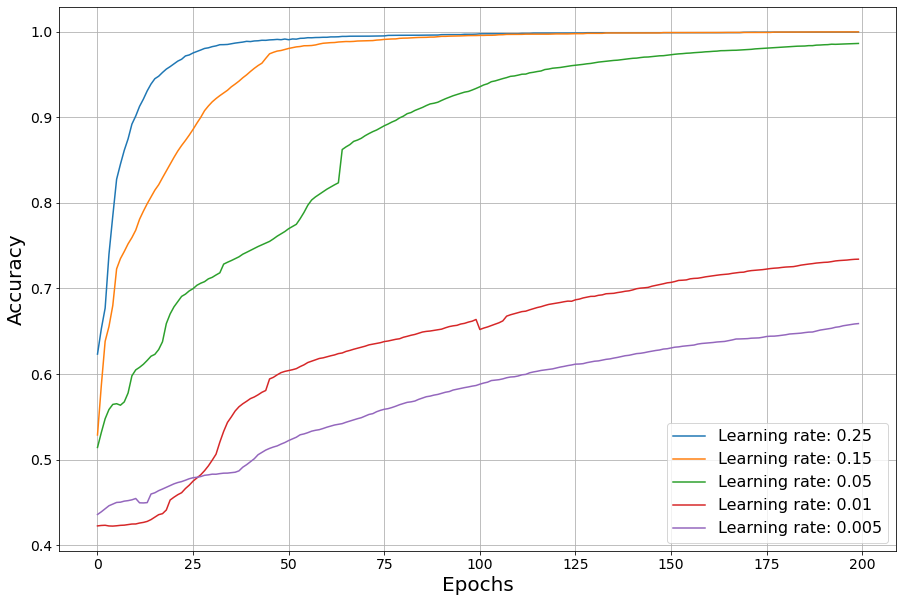
\includegraphics[width=0.49\textwidth]{figs/alphas_acc.png}
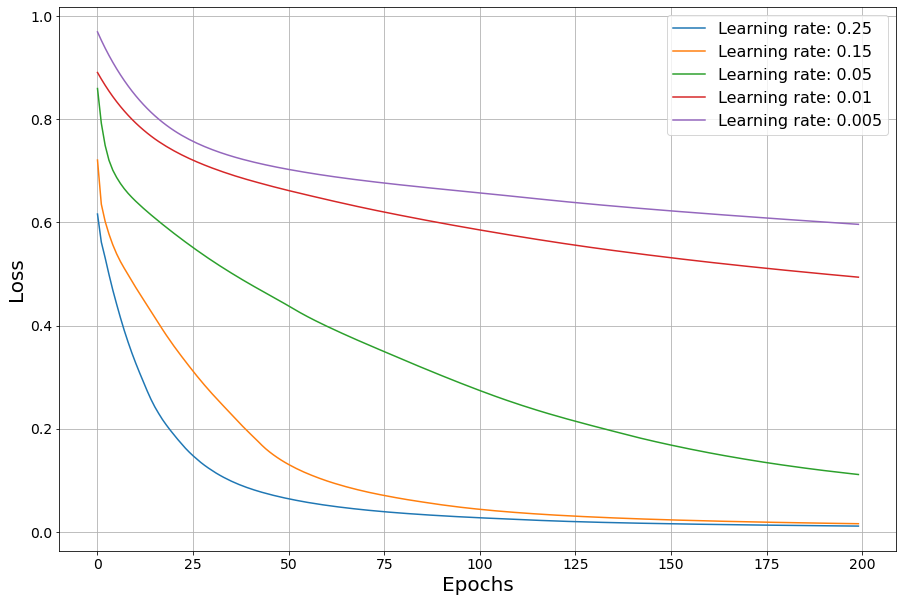
\includegraphics[width=0.49\textwidth]{figs/alphas_loss.png}
\caption{Performance metrics of a neural network during supervised learning with different learning rates.}
\label{fig:perf_alpha}
\end{figure}

Interestingly, when using very small $\alpha$ values, dips in accuracy can be observed. Perhaps, due to the small gradient, the model gets stuck in a local minima, the minima is likely shallow which larger $\alpha$ values have no trouble escaping, hence the lack of dips in accuracy (see if this changes when the train/test sets are introduced (i.e., training set is reduced) which might have an effect on the landscape of the loss function \cite{Guo}).

To make any meaningful conclusion really need to observe how well the model generalises to a test data set.

\section{Discussion and Conclusions}
Sigmoid and Tanh functions are sensitive to input in their mid-point range (where y = 0.5 and y =0.0 respectively), anything below or above theses values quickly reduces the learning rate (output value close to 0 or 1, any changes to weights have very minor impact) and eventually saturates the gradient.
Tanh output range of -1 to 1 has the advantage of adjusting weights in both positive or negative direction in a single iteration as opposed to sigmoid (justification for improved performance of tanh over sigmoid, reference?).
Rectified learning unit function forgoes learning slowdown encountered by sigmoid and tanh when very large inputs are used (ReLU has no upper limit), however negatively weighted inputs cause neurons to die off, stopping learning altogether. Leaky ReLU (an improved version of ReLU) addresses the issue of dying nodes by assigning negative inputs a small negative value (reference?)..

Flatlining - the model gets stuck in a local optima (i.e. surrounded by steep loss function? consider the error landscape, might have saddle/ flat areas which are hard to escape).

In retrospect, implementing adaptive learning rate and alternative weight initialisation approaches (e.g. Xavier) could have benefited to a more robust classifier.

\begin{thebibliography}{10}
\bibitem{Nielsen} Michael A. Nielsen, ``Neural Networks and Deep Learning", Determination Press, 2015
\bibitem{Xavier}Xavier Glorot, Yoshua Bengio, ``Proceedings of the Thirteenth International Conference on Artificial Intelligence and Statistics", PMLR 9:249-256, 2010
\bibitem{Guo}  Yangzi Guo, Adrian Barbu, ``A study of local optima for learning feature interactions using neural networks", 2020

\end{thebibliography}

\end{document}